\documentclass[12pt,letterpaper,noanswers]{exam}
\usepackage[usenames,dvipsnames,svgnames,table]{xcolor}
\usepackage[margin=0.9in]{geometry}
\renewcommand{\familydefault}{\sfdefault}
\usepackage{multicol}
\usepackage{wrapfig}
\pagestyle{head}
\definecolor{c03}{HTML}{FFDDDD}
\header{AM 22b Class 23}{}{Mar 24: Fundamental theorem}
\runningheadrule
\headrule
\usepackage{graphicx} % more modern
\usepackage{amsmath} 
\usepackage{amssymb} 
\usepackage{hyperref}
\usepackage{tcolorbox}
\usepackage[utf8]{inputenc}
\usepackage{diagbox}
\usepackage{graphicx} 
\usepackage{enumitem}
\usepackage{tikz}
\tikzstyle{startstop} = [rectangle, rounded corners, minimum width=3cm, minimum height=1cm,text centered, draw=black]

\tikzstyle{process} = [rectangle, minimum width=3cm, minimum height=1cm, text centered, draw=black, fill=gray!20]
\tikzstyle{decision} = [ellipse, minimum width=3cm, minimum height=0.5cm, text centered, draw=black, fill=white!30]
\tikzstyle{arrow} = [thick,->,>=stealth]
\usetikzlibrary{shapes.geometric, arrows}
\pagenumbering{arabic}

\usepackage[numbered,autolinebreaks,useliterate]{mcode}

\newcommand{\mb}[1]{\underline{#1}}

\begin{document}
 \pdfpageheight 11in 
  \pdfpagewidth 8.5in


\begin{itemize}
% \item There is a pre-class assignment (20 minutes of videos + a few WeBWorK exercises) due at 10am this Monday.  It is available on Canvas.
\itemsep0em
    \item Problem set 06 is due on Thursday March 25th.
    \item Our next quiz will be Friday April 2nd.
    \item There will be a pre-class assignment for Monday March 29th.
   \item The next skill check is for C22, 23, 24 and is on Monday, March 29th.
\end{itemize}

\hrule
\vspace{0.2cm}

% partial derivatives, gradient
% local linearity, differential, directional deriv
% 2nd order partials + equations with partials

\noindent\textbf{Big picture}

In single variable calculus, the fundamental theorem of calculus specifies a relationship between a function and the integral of its derivative.  In multi-variable calculus, a similar theorem exists (and applies to line integrals for some vector fields).  Using that theorem simplifies line integral calculations in the cases where it applies.

\vspace{0.2cm}
\hrule
\vspace{0.2cm}

\noindent\textbf{Skill Check C23 Practice}.  

Let $f = x^2y$ and $\mb F = \nabla f.$  Let $C$ be a path connecting $(0,0)$ to $(1,4)$.  Use the ftcli to find $\int_C \mb F \cdot d\mb r$.


\vspace{0.2cm}
\hrule
\vspace{0.2cm}

\noindent\textbf{Skill Check C23 Practice Solution}.  

The ftcli says $\int_C \nabla f \cdot d\mb r = f(Q) - f(P)$ where path $C$ starts at point $P$ and ends at point $Q$.  We have $P = (0,0)$ and $Q = (1,4)$.  So $\int_C \nabla f \cdot d\mb r = 1^2(4)-0^2(0) = 4$.

\vspace{0.2cm}
\hrule
\vspace{0.2cm}

\noindent\textbf{Teams}
% Dabao, James, Taylor, Akhila, Jonny

\begin{multicols}{2}

1.  student names
\end{multicols}

\vspace{0.2cm}
\hrule
\vspace{0.2cm}



\noindent\textbf{Single variable calculus: fundamental theorem of calculus}. \S 5.3
\begin{tcolorbox}
\begin{itemize}
\itemsep0em
    \item Let $F(x) = \frac{df}{dx}$ on $[a,b]$.  Then $\displaystyle\int_a^b F(x)\ dx = f(b) - f(a)$ by a fundamental theorem of calculus.
    \item Here's some intuition for this: we have $\displaystyle\int_a^b F(x) \ dx = \int_a^b \frac{df}{dx} \ dx$.  The corresponding Riemann sum is $ \sum \frac{df}{dx}\Delta x \approx \displaystyle\sum \Delta f$.  
    
    \item More formally, let $u = f(x)$.  $\displaystyle du = \frac{df}{dx}dx$ (and $\Delta u = \Delta f \approx \frac{df}{dx}\Delta x$).  Doing a change of variables, $\displaystyle\int_a^b \frac{df}{dx}dx = \int_{f(a)}^{f(b)} du =  \left. u \right\vert_{f(a)}^{f(b)} = f(b) - f(a)$ \emph{Notice that the limits of the integral change when we do the change of variables.}
\end{itemize}
\end{tcolorbox}

\noindent\textbf{Example}.

Let $f(x) = x^3 + x$.  Differentiate $f(x)$.  Use the fundamental theorem of calculus to find $\displaystyle\int_0^2 \left(3x^2 + 1\right)\ dx$.

\vspace{1in}


\noindent\textbf{Question}.

How might you generalize the fundamental theorem of calculus to an integral along a path in 3-space?

\eject


\vspace{0.2cm}
\hrule
\vspace{0.2cm}
\noindent\textbf{Line integrals and the fundamental theorem} \S 18.3
\begin{tcolorbox}
\begin{itemize}
\itemsep0em
    \item For $C$ a piecewise smooth oriented path with starting point $P$ and ending point $Q$, and $f$ a function whose gradient is continuous on $C$, the \textbf{fundamental theorem of calculus for line integrals} (ftcli) states that \[\int_C f_{\mb T}\ ds =f(Q)-f(P)\] where  $f_{\mb T} = \nabla f \cdot \mb{T},$ with $\mb T$ a unit tangent vector in the direction of motion along curve $C$.
    \item Intuition: $\displaystyle\int_C \nabla f \cdot \mb T\ ds = \int_C f_{\mb T}\ ds$.  $f_{\mb T}$ is the directional derivative of $f$ in the direction tangent to the curve, so gives the rate of change of $f$ with respect to distance along the curve.  We have $\Delta f\approx f_{\mb T}\Delta s$  The integral is approximately $\displaystyle\sum_i f_{\mb T}\Delta s \approx \sum_i \Delta f$ so this is essentially $\int_C df$, or the change in the function from the beginning to the end of the curve.
    \item In the single variable setting, an arbitrary function $f(x)$ had an antiderivative $\int f(x) dx$.  From the FTCLI we see that only certain vector fields have an "anti-derivative" (with the term used loosely): vector fields that represent the derivative of a function.
\end{itemize}

\end{tcolorbox}


 \noindent\textbf{Gradient vector fields} \S 18.3
\begin{tcolorbox}
\begin{itemize}
\itemsep0em
    \item A \textbf{gradient field} is a vector field $\mb F$ where $\mb F = \nabla f$ for some scalar function $f$. 
    \item The function $f$ is called a \textbf{potential function} for the vector field $\mb F$.
\end{itemize}
\end{tcolorbox}


% \noindent\textbf{Example (gradient field)} A gradient field, $\mb F = \mb \nabla f = f_x\mb i + f_y\mb j$, is shown, along with contours of the function $f$, in the figure below.

% 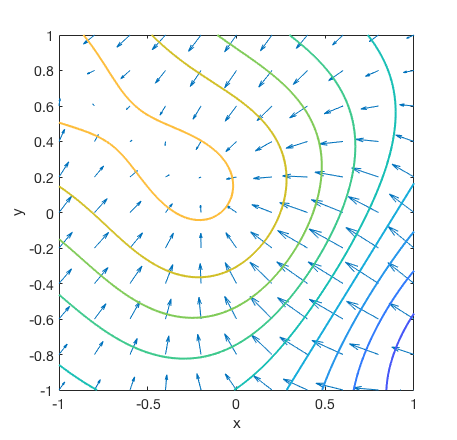
\includegraphics[width=2in]{img/C26p2-18.png}


\noindent\textbf{Examples: matching}

Match each potential function with its gradient field.  %\emph{pollQ}

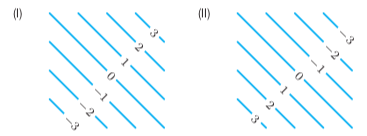
\includegraphics[width=0.45\linewidth]{img/C22p1a.png}
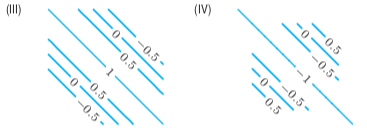
\includegraphics[width=0.45\linewidth]{img/C22p1b.png}

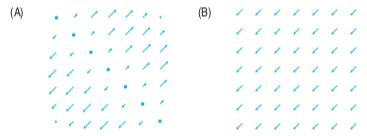
\includegraphics[width=0.45\linewidth]{img/C22p1c.png}

\includegraphics[width=0.45\linewidth]{img/C22p1d.png}
\vspace{1in}


\eject

\noindent\textbf{Example (use the ftcli)}.  Let $f = xy$ and $\mb F = \nabla f.$  Let $C$ be a sinusoidal path connecting $(0,0)$ to $(3\pi/2,-1)$.  Use the ftcli to find $\int_C \nabla f \cdot d\mb r$.


\vspace{1.2in}

%\eject
\vspace{0.2cm}
\hrule
\vspace{0.2cm}
\noindent\textbf{Gradient fields are equivalent to path independent vector fields} \S 18.3
\begin{tcolorbox}
\begin{itemize}
\itemsep0em
    \item A vector field is called \textbf{path independent} or \textbf{conservative} if, for any two points $P$ and $Q$, the line integral $\displaystyle\int_C \mb F\cdot d\mb r$ has the same value along any piecewise smooth path $C$ from $P$ to $Q$ lying in the domain of $\mb F$.  
    \item Continuous gradient fields are path independent vector fields: It is straightforward to show that gradient field $\Longrightarrow$ path independent vector field, so long as $\nabla f$ is continuous on every path $C$ in the domain of $\nabla f$.  See \S 18.3 of the text for an argument showing that if $\mb F$ is a continuous path-independent vector field on an open region $R$, then $\mb F = \nabla f$ for some $f$ defined on $R$.  \emph{Notice that $f$ needs to be defined on $R$, not just a subset of $R$.}
    \item The term \textbf{conservative} is used in physics to refer to path independent force vector fields.  For example, the gravitational force is called conservative.
\end{itemize}
\end{tcolorbox} 

%\includegraphics[width=4in]{img/N27p1.png}

\noindent\textbf{Example (path independent)} The figure below shows a vector field $\nabla f$ where $f$ is continuously differentiable in the whole plane.  The ends of the oriented curve $C$ from $P$ to $Q$ are shown but the middle portion of the curve is not shown.  If possible, find the sign of $\int_C \mb\nabla f\cdot d\mb r$.

\emph{pollQ}

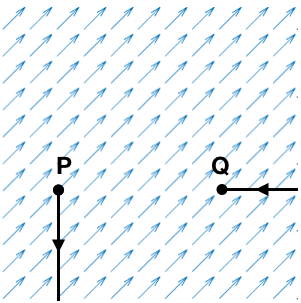
\includegraphics[width=2.5in]{img/C26p1-18.png}

\eject

\vspace{0.2cm}
\hrule
\vspace{0.2cm}


\noindent\textbf{Path independent vector fields are equivalent to circulation-free vector fields} \S 18.3
\begin{tcolorbox}
\begin{itemize}
\itemsep0em
    \item A vector field is called \textbf{circulation free} when $\displaystyle\oint_C \mb F\cdot d\mb r = 0$ for all curves $C$ in the domain of $\mb F$.
    \item The term circulation-free is used in engineering applications, particularly to describe velocity vectors fields in fluids.
\end{itemize}
\end{tcolorbox} 



\noindent\textbf{Example (circulation free)}.  Let $\mb F$ be a path independent vector field.  Let $C$ be a simple closed curve with negative orientation (clockwise) with $P$ and $Q$ two distinct points on the curve.  Let $C_1$ and $C_2$ be paths from $P$ to $Q$ with orientations as shown in the figure below.

\begin{multicols}{2}
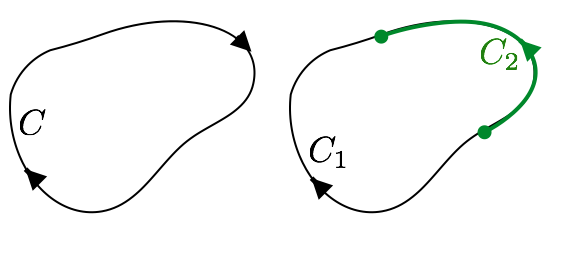
\includegraphics[width=2.5in]{img/C27p2.png}

Rewrite $\displaystyle\oint_C \mb F\cdot d\mb r$  using $C_1$ and $C_2$.  \emph{pollQ}
\end{multicols}
\vspace{0.5in}




% \vfill

% \noindent\textbf{Path independent field = gradient field}.  Gradient vector fields are always path-independent vector fields.  Are path-independent vector fields always gradient fields? (Yes).

% Given a path-independent vector field, choose a point $P_0$ to be the \emph{ground}, with the potential $f(P_0) = 0$.  Let $f(Q) = \int_C \mb F\cdot d\mb r$ where $C$ is a path from $P_0$ to $Q$ (and $f(Q)$ is the work done by the vector field in moving an object from $P_0$ to $Q$).

% If $\mb\nabla f = \mb F$ then $\mb F$ is a gradient field.  The course text has a careful argument in section 18.3 (see text for details) showing that $\mb\nabla f = \mb F$, so path-independent vector fields are always gradient fields.

% \vfill

\vspace{0.2cm}
\hrule
\vspace{0.2cm}


\noindent\textbf{Constructing a potential function}
\begin{tcolorbox}
\begin{itemize}
    \item Given a vector field, $\nabla f$, we can construct a potential function, $f$.
    \item Given $\nabla f= \langle P,Q,R\rangle$, we have $P =f_x, Q=f_y, R=f_z$.  
\begin{enumerate}
    \item Let $f = \int P dx + g(y,z)$ where $g(y,z)$ is an unknown function of $y$ and $z$.  
    \item We have $f_y = \frac{\partial}{\partial y}\int P dx + g_y(y,z)$.  Assume $f_y = Q$ and rearrange to find $g_y(y,z)$.
    \item We now have $f = \int P dx + \int g_y dy + h(z)$.
    \item We have $f_z = \frac{\partial}{\partial z}\left(\int P dx +\int g_y dy \right)+ h_z$. Assume $f_z = R$ and rearrange to find $h_z$.
    \item Let $f = \int P dx + \int g_y dy + \int h_z dz$.  This is a possible potential function for the vector field.
\end{enumerate} 
\end{itemize}
\end{tcolorbox}
\noindent\textbf{Example (2d)}

Find $f$ if $\nabla f = \langle 2xy, x^2+y\rangle$.

\begin{enumerate}
    \item Let $f = \int 2xy dx + g(y) = x^2y + g(y)$.
    \item $f_y = x^2 + g_y = x^2+2y$, so $g_y = 2y$.
    \item $f = x^2y + \int 2ydy = x^2y + y^2$ works as a potential function.  $f=x^2y+y^2+3$ would work as well.
\end{enumerate}

\noindent\textbf{Example}
Calculate the line integral $\int_C \nabla f \cdot d\mb r$ exactly, where $\displaystyle\nabla f = \left\langle 2xe^{x^2+yz}, ze^{x^2+yz}, ye^{x^2+yz}\right\rangle$ and $C$ is a curve in the plane $z=0$ as shown below.

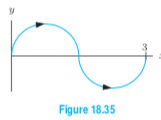
\includegraphics{img/C22p2.png}


\vfill

\noindent\textbf{Problem}.  Let $\mb r = x\mb i + y\mb j + z\mb k$ and $\mb a = a_1\mb i + a_2\mb j + a_3\mb k$.  Let $C$ be a path from the origin to the point with position vector $\mb r_0$.  Find $\int_C \nabla(\mb r\cdot \mb a)\cdot d\mb r$.  What is the maximum possible value of this line integral if $\Vert \mb r_0\Vert = 10?$
\vfill




\vspace{0.2cm}
\hrule
\vspace{0.2cm}


\end{document}